\documentclass[aspectratio=169,10pt]{beamer}

\usetheme[progressbar=frametitle, numbering=fraction]{metropolis}
\usepackage{tikz}
\usetikzlibrary{positioning, arrows.meta, shapes.geometric}
\usepackage{xcolor}

% ---------------------------------------------------------------- colours
\definecolor{accent}{HTML}{1F6FB2}
\definecolor{warn}{HTML}{C0392B}
\definecolor{ok}{HTML}{2E8B57}
\definecolor{soft}{HTML}{EEF3F8}
\setbeamercolor{frametitle}{bg=accent!85!black}
\setbeamercolor{progress bar}{fg=accent!60, bg=accent!15}
\setbeamercolor{alerted text}{fg=warn}

% ---------------------------------------------------------------- helpers
\newcommand{\ui}[1]{\textbf{#1}}                 % UI labels
\newcommand{\cmd}[1]{\texttt{#1}}               % file names, values
\newcommand{\key}[1]{\tikz[baseline=(k.base)]\node[draw, rounded corners=2pt,
  inner sep=2pt, fill=soft, font=\ttfamily\small](k){#1};}

\newcommand{\reportbox}[1]{%
  \begin{tikzpicture}
    \node[fill=warn!10, draw=warn!70, rounded corners=3pt, inner sep=6pt,
          text width=0.9\linewidth, font=\small]
      {\textcolor{warn}{\textbf{Report to the operator:}} #1};
  \end{tikzpicture}}

\newcommand{\checkbox}[1]{%
  \begin{tikzpicture}
    \node[fill=ok!10, draw=ok!70, rounded corners=3pt, inner sep=6pt,
          text width=0.9\linewidth, font=\small]
      {\textcolor{ok}{\textbf{Check:}} #1};
  \end{tikzpicture}}

\newcommand{\stepno}[1]{%
  \tikz[baseline=(s.base)]\node[circle, fill=accent, text=white,
  inner sep=1.5pt, minimum size=1.3em, font=\bfseries\small](s){#1};}

% ---------------------------------------------------------------- meta
\title{Tutorial Guide (Windows~11)}
\subtitle{From a zip of container images to a live substation on the hub}
\author{Lablink Hands-on Tutorial}
\date{}

\begin{document}

\maketitle

% ================================================================ overview
\begin{frame}{What you get and what you do}
  \begin{columns}[T]
    \begin{column}{0.48\textwidth}
      \textbf{You receive}
      \begin{itemize}
        \item A zip of container images
        \item From the hub operator:
          \begin{itemize}
            \item network details
            \item your \cmd{OPCUA\_CONFIG} value
            \item the go-ahead for each stage
          \end{itemize}
      \end{itemize}
      \vspace{0.3em}
      \textbf{Ground rules}
      \begin{itemize}
        \item Talk to the operator whenever a step says \emph{report}
        \item Nothing to type in a terminal beyond what the steps name
      \end{itemize}
    \end{column}
    \begin{column}{0.48\textwidth}
      \textbf{The eleven steps}
      \footnotesize
      \begin{enumerate}\setlength{\itemsep}{0pt}
        \item Join the tutorial network
        \item Report your IPv4 address
        \item Open the hub
        \item Unpack the archive
        \item Start Docker Desktop
        \item Load the images
        \item Confirm the images
        \item Run the substation
        \item Check the substation page
        \item Run the OPC UA client
        \item Move the slider, watch the hub
      \end{enumerate}
    \end{column}
  \end{columns}
\end{frame}

% ================================================================ architecture
\begin{frame}{The setup at a glance}
  \centering
  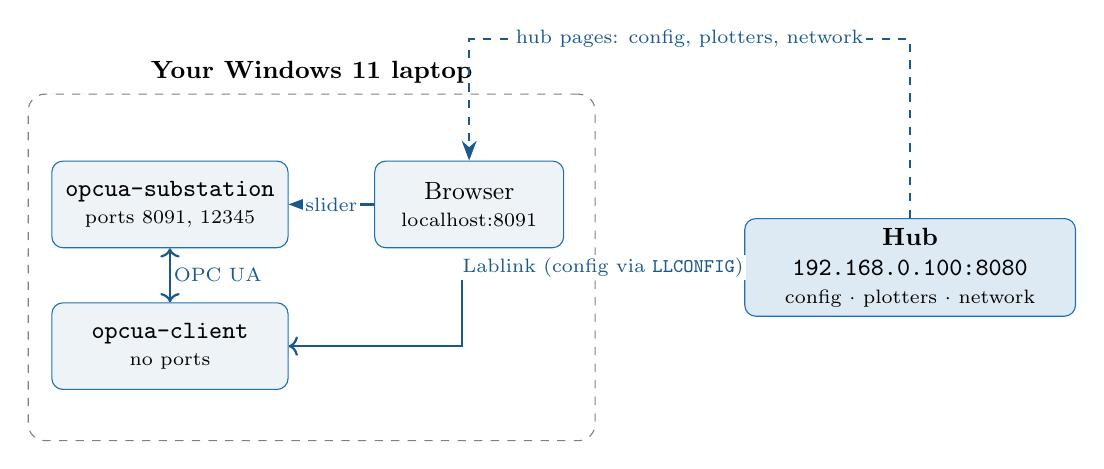
\begin{tikzpicture}[
      box/.style={draw, rounded corners=4pt, align=center, minimum height=1.1cm,
                  font=\small, fill=soft, draw=accent},
      hub/.style={box, fill=accent!15, minimum width=4.2cm},
      arr/.style={-{Stealth[length=2.5mm]}, thick, accent!80!black},
      lbl/.style={font=\scriptsize, midway, fill=white, inner sep=1pt}]
    % station
    \node[draw=gray, dashed, rounded corners=6pt, minimum width=7.2cm,
          minimum height=4.4cm, label={[font=\small\bfseries]above:Your Windows~11 laptop}]
          (laptop) at (0,0) {};
    \node[box, minimum width=3cm] (sub) at (-1.8,0.8)
         {\cmd{opcua-substation}\\[-1pt]\scriptsize ports 8091, 12345};
    \node[box, minimum width=3cm] (cli) at (-1.8,-1.0)
         {\cmd{opcua-client}\\[-1pt]\scriptsize no ports};
    \node[box, minimum width=2.4cm] (brw) at (2.0,0.8)
         {Browser\\[-1pt]\scriptsize localhost:8091};
    % hub
    \node[hub] (h) at (7.6,0)
         {\textbf{Hub}\\ \cmd{192.168.0.100:8080}\\[-1pt]
          \scriptsize config $\cdot$ plotters $\cdot$ network};
    \draw[arr] (brw) -- node[lbl]{slider} (sub);
    \draw[arr, <->] (cli) -- node[lbl, right]{OPC UA} (sub);
    \draw[arr, <->] (cli.east) -- ++(2.2,0) |- node[lbl, pos=0.75]{Lablink (config via \texttt{LLCONFIG})} (h.west);
    \draw[arr, dashed] (h.north) |- node[lbl, pos=0.75]{hub pages: config, plotters, network} (brw.north |- 0,2.9) -- (brw.north);
  \end{tikzpicture}
\end{frame}

% ================================================================ part 1
\section{Connect to the hub}

\begin{frame}{\stepno{1}\ Join the tutorial network}
  \begin{itemize}
    \item Use the Wi-Fi name and password, or the Ethernet instructions,
          that the hub operator gives you.
    \item Wait until Windows shows the network as \ui{connected}.
  \end{itemize}
\end{frame}

\begin{frame}{\stepno{2}\ Read your IPv4 address}
  \begin{enumerate}
    \item Press \key{Win} + \key{I}. Settings opens.
    \item Open \ui{Network \& internet}.
    \item Open the connected \ui{Wi-Fi} or \ui{Ethernet} entry,
          then the name of the network you just joined.
    \item Read \ui{IPv4 address}.
  \end{enumerate}
  \vfill
  \reportbox{say your IPv4 address. Wait until they confirm the hub knows your machine.}
\end{frame}

\begin{frame}{\stepno{3}\ Open the hub}
  In a browser, go to \alert{\cmd{http://192.168.0.100:8080}}\\
  {\small (or the address the operator gave you).}

  \vspace{0.8em}
  The page title is \ui{Lablink Hands-on Tutorial}. Open each link and confirm it loads:
  \vspace{0.3em}

  \begin{columns}[T]
    \begin{column}{0.55\textwidth}
      \small
      \begin{tabular}{@{}ll@{}}
        \ui{Configuration server}   & \cmd{/config/} \\
        \ui{Supply temperature}     & \cmd{/plot/tsupply/} \\
        \ui{Supply mass flow}       & \cmd{/plot/mflow/} \\
        \ui{Substation temperature} & \cmd{/plot/tsub/} \\
        \ui{Network display}        & \cmd{/network/} \\
      \end{tabular}
    \end{column}
    \begin{column}{0.42\textwidth}
      \checkbox{Leave this tab open. You come back to it at the end.}
    \end{column}
  \end{columns}
\end{frame}

% ================================================================ part 2
\section{Prepare Docker}

\begin{frame}{\stepno{4}\ Unpack the archive with 7-Zip}
  The operator gives you \cmd{lablink-station-images.zip}.
  \begin{enumerate}
    \item Right-click the zip.
    \item Choose \ui{7-Zip $\rightarrow$ Extract to ``lablink-station-images$\backslash$''}.
  \end{enumerate}
  \vspace{0.6em}
  The new folder contains:
  \begin{center}
    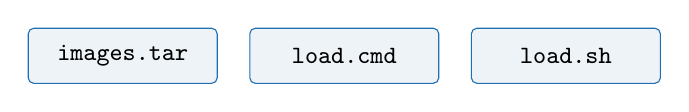
\begin{tikzpicture}[f/.style={draw=accent, fill=soft, rounded corners=2pt,
                         font=\ttfamily\small, minimum width=2.4cm, minimum height=0.7cm}]
      \node[f] (a) {images.tar};
      \node[f, right=0.4cm of a] (b) {load.cmd};
      \node[f, right=0.4cm of b] (c) {load.sh};
    \end{tikzpicture}
  \end{center}
\end{frame}

\begin{frame}{\stepno{5}\ Start Docker Desktop}
  \begin{itemize}
    \item Start \ui{Docker Desktop}.
    \item Wait until the whale menu says the \ui{engine is running}.
    \item If Windows Firewall asks, allow Docker on \ui{private networks}.
  \end{itemize}
\end{frame}

\begin{frame}{\stepno{6}\ Load the images}
  \begin{itemize}
    \item In the extracted folder, double-click \cmd{load.cmd}.
    \item A command window runs \cmd{docker load} on \cmd{images.tar}.
    \item The window closes by itself when the load finishes.
          A large archive can take about a minute.
  \end{itemize}
  \vfill
  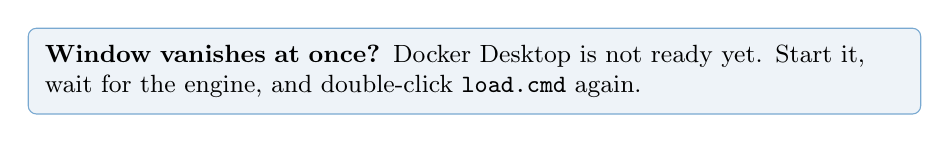
\begin{tikzpicture}
    \node[fill=soft, draw=accent!60, rounded corners=3pt, inner sep=6pt,
          text width=0.9\linewidth, font=\small]
      {\textbf{Window vanishes at once?} Docker Desktop is not ready yet.
       Start it, wait for the engine, and double-click \cmd{load.cmd} again.};
  \end{tikzpicture}
\end{frame}

\begin{frame}{\stepno{7}\ Confirm the images}
  In Docker Desktop, open \ui{Images}. Both are listed:
  \vspace{0.6em}
  \begin{center}
    \begin{tabular}{ll}
      \hline
      \textbf{Image} & \textbf{Tag} \\
      \hline
      \cmd{lablink-workshop/opcua-substation} & \cmd{latest} \\
      \cmd{ait1/lablink-opcua-client}         & \cmd{latest} \\
      \hline
    \end{tabular}
  \end{center}
  \vfill
  \reportbox{if either image is missing.}
\end{frame}

% ================================================================ part 3
\section{Run the station}

\begin{frame}{\stepno{8}\ Run the substation}
  In \ui{Images}, on \cmd{lablink-workshop/opcua-substation}, click \ui{Run}. Set:
  \vspace{0.4em}
  \begin{columns}[T]
    \begin{column}{0.55\textwidth}
      \small
      \begin{tabular}{@{}ll@{}}
        \ui{Container name} & \cmd{opcua-substation} \\[3pt]
        \ui{Ports}          & host \cmd{8091} $\rightarrow$ container \cmd{80} \\
                            & host \cmd{12345} $\rightarrow$ container \cmd{12345} \\[3pt]
        \ui{Volumes}        & leave empty \\
      \end{tabular}
    \end{column}
    \begin{column}{0.42\textwidth}
      \small
      Add a second port row if the dialog shows only one.
      Set the host ports yourself.
    \end{column}
  \end{columns}
  \vfill
  \checkbox{Click \ui{Run}. In \ui{Containers}, \cmd{opcua-substation} stays running.}
\end{frame}

\begin{frame}{\stepno{9}\ Check the substation page}
  Open \alert{\cmd{http://localhost:8091}}. You see:
  \begin{itemize}
    \item \ui{Substation display}
    \item the instrument dials
    \item the \ui{heat load setpoint} slider, scale \textbf{20\,kW} to \textbf{80\,kW}
  \end{itemize}
  \vfill
  \reportbox{if the page does not load.}
\end{frame}

\begin{frame}{\stepno{10}\ Run the OPC UA client}
  In \ui{Images}, on \cmd{ait1/lablink-opcua-client}, click \ui{Run}. Set:
  \vspace{0.3em}
  \small
  \begin{tabular}{@{}ll@{}}
    \ui{Container name} & \cmd{opcua-client} \\
    \ui{Ports}          & leave empty \\
    \ui{Environment}    & \cmd{LLCONFIG} = \cmd{http://192.168.0.100:8080/config/get?id=} \\
                        & \cmd{OPCUA\_CONFIG} = \emph{string from the operator} \\
  \end{tabular}

  \vspace{0.5em}
  \cmd{LLCONFIG} ends with \alert{\cmd{?id=}}. With a different hub address,
  swap the address and keep \cmd{/config/get?id=}.

  \vspace{0.5em}
  \checkbox{\cmd{opcua-client} stays running, and the dials on
            \cmd{localhost:8091} show live values.}

  \vspace{0.2em}
  \reportbox{if \cmd{opcua-client} stops. When they say the hub is ready,
             press the container's start button.}
\end{frame}

% ================================================================ part 4
\section{See it work}

\begin{frame}{\stepno{11}\ Move the heat-load slider, watch the hub}
  \begin{enumerate}
    \item On \cmd{localhost:8091}, drag \ui{heat load setpoint} somewhere
          between 20\,kW and 80\,kW and release it.
    \item Switch to the hub tab from step~3.
    \item Open \ui{Network display} and the three plotters.
  \end{enumerate}
  \vspace{0.4em}
  \begin{center}
    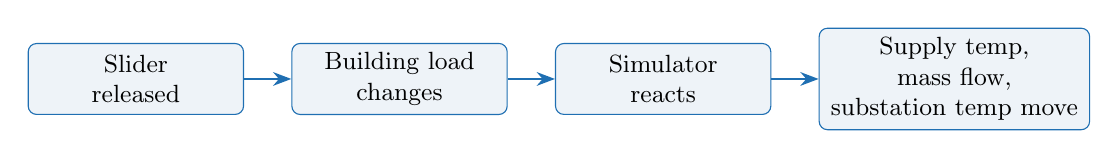
\begin{tikzpicture}[n/.style={draw=accent, fill=soft, rounded corners=3pt,
                         font=\small, align=center, minimum height=0.9cm, text width=2.5cm},
                        a/.style={-{Stealth}, thick, accent}]
      \node[n] (s) {Slider\\released};
      \node[n, right=0.6cm of s] (l) {Building load\\changes};
      \node[n, right=0.6cm of l] (sim) {Simulator\\reacts};
      \node[n, right=0.6cm of sim, text width=3.2cm] (t)
           {Supply temp, mass flow,\\substation temp move};
      \draw[a] (s) -- (l); \draw[a] (l) -- (sim); \draw[a] (sim) -- (t);
    \end{tikzpicture}
  \end{center}
  \vfill
  \reportbox{if nothing on the hub changes: the slider value you set and
             which pages stayed still.}
\end{frame}

% ================================================================ cheat sheet
\begin{frame}{Cheat sheet}
  \small
  \begin{columns}[T]
    \begin{column}{0.5\textwidth}
      \textbf{Addresses}\\[2pt]
      \begin{tabular}{@{}ll@{}}
        Hub          & \cmd{http://192.168.0.100:8080} \\
        Substation   & \cmd{http://localhost:8091} \\
      \end{tabular}

      \vspace{0.8em}
      \textbf{Images (tag \cmd{latest})}\\[2pt]
      \cmd{lablink-workshop/opcua-substation}\\
      \cmd{ait1/lablink-opcua-client}
    \end{column}
    \begin{column}{0.48\textwidth}
      \textbf{Containers}\\[2pt]
      \cmd{opcua-substation}\\
      \quad 8091$\rightarrow$80, 12345$\rightarrow$12345\\[4pt]
      \cmd{opcua-client}\\
      \quad no ports\\
      \quad \cmd{LLCONFIG} $=\ \ldots$\cmd{/config/get?id=}\\
      \quad \cmd{OPCUA\_CONFIG} $=$ from operator
    \end{column}
  \end{columns}
\end{frame}

\end{document}
